\documentclass[12pt,a4paper]{article}

% ─── Page Layout ───────────────────────────────────────────────────────────────
\usepackage[a4paper, margin=0.8in, headheight=14pt]{geometry}

% ─── Fonts (XeLaTeX) ───────────────────────────────────────────────────────────
\usepackage{fontspec}
\usepackage{unicode-math}
\setmainfont{TeX Gyre Pagella}
\setmonofont[Scale=0.88]{TeX Gyre Cursor}
\setmathfont{Latin Modern Math}

% ─── Packages ──────────────────────────────────────────────────────────────────
\usepackage{xcolor}
\usepackage{colortbl}
\usepackage{titlesec}
\usepackage{enumitem}
\usepackage{tabularx}
\usepackage{booktabs}
\usepackage{array}
\usepackage{amsmath}
\usepackage{tikz}
\usetikzlibrary{shapes.geometric, arrows.meta, positioning, calc, fit, decorations.pathreplacing}
\usepackage{tcolorbox}
\tcbuselibrary{skins, breakable}
\usepackage{hyperref}
\usepackage{fancyhdr}
\usepackage{graphicx}
\usepackage{microtype}
\hyphenpenalty=10000
\exhyphenpenalty=10000
\sloppy
\usepackage{caption}
\usepackage{setspace}
\usepackage{multirow}
\usepackage{tocloft}

% ─── Q&A helper ────────────────────────────────────────────────────────────────
\newcommand{\Q}[1]{\textbf{#1}\par\noindent\ignorespaces}

% ─── Colour Palette ────────────────────────────────────────────────────────────
\definecolor{myred}{RGB}{196,30,58}
\definecolor{mydark}{RGB}{30,30,50}
\definecolor{mygreen}{RGB}{14,120,80}
\definecolor{myteal}{RGB}{0,130,140}
\definecolor{myamber}{RGB}{180,100,0}
\definecolor{mypurple}{RGB}{100,30,160}
\definecolor{mygray}{RGB}{246,247,249}
\definecolor{mgframe}{RGB}{180,185,200}
\definecolor{watermark}{RGB}{145,150,170}
\definecolor{hdrred}{RGB}{250,232,235}
\definecolor{hdrgreen}{RGB}{220,244,233}
\definecolor{hdrteal}{RGB}{220,242,244}
\definecolor{hdramber}{RGB}{253,242,215}
\definecolor{hdrpurple}{RGB}{238,228,255}
\definecolor{hdrgray}{RGB}{238,240,245}
\definecolor{rowalt}{RGB}{250,251,253}

% ─── Section Formatting ────────────────────────────────────────────────────────
\titleformat{\section}
  {\large\bfseries\color{myred}}{\thesection.}{0.5em}{}
  [\vspace{1pt}{\color{myred}\rule{\linewidth}{0.8pt}}]
\titleformat{\subsection}
  {\normalsize\bfseries\color{myteal}}{\thesubsection}{0.5em}{}
\titlespacing*{\section}{0pt}{18pt}{7pt}
\titlespacing*{\subsection}{0pt}{11pt}{4pt}

% ─── Paragraph ─────────────────────────────────────────────────────────────────
\setlength{\parindent}{0pt}
\setlength{\parskip}{4pt}

% ─── TOC Styling ───────────────────────────────────────────────────────────────
\renewcommand{\cfttoctitlefont}{\large\bfseries\color{myred}}
\renewcommand{\cftaftertoctitle}{\par\noindent{\color{myred}\rule{\linewidth}{0.8pt}}}
\setlength{\cftbeforetoctitleskip}{0pt}
\setlength{\cftaftertoctitleskip}{6pt}
\renewcommand{\cftsecfont}{\normalsize\bfseries\color{mydark}}
\renewcommand{\cftsecpagefont}{\normalsize\bfseries\color{mydark}}
\renewcommand{\cftsecleader}{\cftdotfill{\cftdotsep}}
\setlength{\cftbeforesecskip}{7pt}
\renewcommand{\cftsubsecfont}{\small\color{mydark}}
\renewcommand{\cftsubsecpagefont}{\small\color{mydark}}
\setlength{\cftbeforesubsecskip}{3pt}
\setlength{\cftsubsecindent}{1.4em}

% ─── Table helpers ─────────────────────────────────────────────────────────────
\renewcommand{\arraystretch}{1.45}
\setlength{\tabcolsep}{6pt}
\arrayrulecolor{mydark}
\newcolumntype{B}[1]{>{\small\bfseries\raggedright\arraybackslash}m{#1}}
\newcolumntype{Y}{>{\small\raggedright\arraybackslash}X}
\renewcommand{\tabularxcolumn}[1]{m{#1}}

% ─── Header / Footer ───────────────────────────────────────────────────────────
\pagestyle{fancy}
\fancyhf{}
\fancyhead[L]{\small\color{myred}\textbf{EC501}\;\color{mydark}--- Electromagnetic Waves}
\fancyhead[R]{\small\color{myteal}\textbf{Module 1 Notes}}
\fancyfoot[C]{\small\color{mydark}\thepage}
\fancyfoot[R]{\small\color{watermark}\textit{\copyright\ Biraj}}
\renewcommand{\headrulewidth}{0.5pt}
\renewcommand{\footrulewidth}{0.3pt}

% ─── Hyperref ──────────────────────────────────────────────────────────────────
\hypersetup{
  colorlinks=true, linkcolor=myteal, urlcolor=myteal,
  pdfauthor={Biraj Sarkar},
  pdftitle={EC501 --- Module 1 Notes}
}

% ─── tcolorbox styles ──────────────────────────────────────────────────────────
\tcbset{
  tikzbox/.style={
    colback=mygray, colframe=mgframe, boxrule=0.6pt, arc=4pt,
    left=8pt, right=8pt, top=6pt, bottom=6pt,
    colbacktitle=mgframe, coltitle=mydark,
    fonttitle=\small\bfseries
  },
  defbox/.style={
    colback=hdrgreen, colframe=mygreen, boxrule=0.8pt, arc=4pt,
    left=9pt, right=9pt, top=6pt, bottom=6pt,
    colbacktitle=mygreen, coltitle=white,
    fonttitle=\small\bfseries
  },
  formulabox/.style={
    colback=hdrteal, colframe=myteal, boxrule=0.8pt, arc=4pt,
    left=9pt, right=9pt, top=7pt, bottom=7pt,
    colbacktitle=myteal, coltitle=white,
    fonttitle=\small\bfseries
  },
  examplebox/.style={
    colback=hdramber, colframe=myamber, boxrule=0.8pt, arc=4pt,
    left=9pt, right=9pt, top=6pt, bottom=6pt,
    colbacktitle=myamber, coltitle=white,
    fonttitle=\small\bfseries
  },
  masonbox/.style={
    colback=hdrpurple, colframe=mypurple, boxrule=0.8pt, arc=4pt,
    left=9pt, right=9pt, top=6pt, bottom=6pt,
    colbacktitle=mypurple, coltitle=white,
    fonttitle=\small\bfseries
  },
  exambox/.style={
    colback=hdrpurple, colframe=mypurple, boxrule=1pt, arc=5pt,
    left=10pt, right=10pt, top=8pt, bottom=8pt,
    colbacktitle=mypurple, coltitle=white,
    fonttitle=\bfseries,
    breakable, title after break={\textbf{Frequently Asked / Viva Questions (contd.)}}}
}
% Make all boxes breakable across pages
\tcbset{breakable}

% ─── TikZ styles ───────────────────────────────────────────────────────────────
\tikzset{
  block/.style={rectangle, draw=myteal, fill=hdrteal,
    text width=2.4cm, align=center, minimum height=0.95cm,
    font=\small, rounded corners=3pt, line width=0.7pt},
  redblock/.style={rectangle, draw=myred, fill=hdrred,
    text width=2.4cm, align=center, minimum height=0.95cm,
    font=\small, rounded corners=3pt, line width=0.7pt},
  netnode/.style={rectangle, draw=myteal, fill=hdrteal,
    text width=1.5cm, align=center, minimum height=0.8cm,
    font=\small, rounded corners=3pt, line width=0.7pt},
  sumjunc/.style={circle, draw=myamber, fill=hdramber,
    minimum size=0.62cm, font=\small, line width=0.8pt},
  snode/.style={circle, draw=mypurple, fill=hdrpurple,
    minimum size=0.55cm, font=\footnotesize, line width=0.7pt},
  arrow/.style={-Stealth, thick, color=mydark},
  redarrow/.style={-Stealth, thick, color=myred},
  line/.style={thick, color=mydark}
}

% ═══════════════════════════════════════════════════════════════════════════════
\begin{document}
% ═══════════════════════════════════════════════════════════════════════════════

\begin{center}
  {\LARGE\bfseries\color{myred} EC501 --- Electromagnetic Waves}\\[5pt]
  {\normalsize\color{mydark} Semester V \quad$\bullet$\quad 3L:0T:0P \quad$\bullet$\quad 3 Credits}\\[3pt]
  {\normalsize\color{myteal}\textbf{Module 1 Exam Notes: Vectors, Maxwell Equations and Boundaries}}\\[3pt]
  {\small\color{mydark} CGEC \;$|$\; B.Tech ECE (2023--27) \;$|$\; \textit{Biraj Sarkar}}
\end{center}
\vspace{2pt}
\noindent{\color{myred}\rule{\linewidth}{1.5pt}}
\vspace{2pt}

\hypersetup{linkcolor=mydark}
\tableofcontents
\hypersetup{linkcolor=myteal}
\newpage

\section{Vectors and Vector Calculus}
\begin{tcolorbox}[defbox,title={Scalars, vectors and fields}]
A scalar has magnitude only. A vector has magnitude and direction. A field assigns a scalar or vector value to each point in a region.
\end{tcolorbox}
\begin{itemize}[leftmargin=*,itemsep=3pt]
\item \textbf{Components.} Write $\mathbf A=A_x\hat{\mathbf x}+A_y\hat{\mathbf y}+A_z\hat{\mathbf z}$. Its magnitude is $\sqrt{A_x^2+A_y^2+A_z^2}$ and its unit vector is $\mathbf A/|\mathbf A|$.
\item \textbf{Dot product.} $\mathbf A\cdot\mathbf B=\sum_i A_i B_i=|\mathbf A||\mathbf B|\cos\theta$. Use it for a projection or normal flux.
\item \textbf{Cross product.} The magnitude is $|\mathbf A||\mathbf B|\sin\theta$ with right-hand direction. Its $x$ component is $A_yB_z-A_zB_y$. Cycle $x,y,z$ for the others.
\item \textbf{Coordinates.} In cylindrical coordinates, $x=\rho\cos\phi$, $y=\rho\sin\phi$ and $dV=\rho\,d\rho\,d\phi\,dz$. In spherical coordinates, $\rho=r\sin\theta$, $z=r\cos\theta$ and $dV=r^2\sin\theta\,dr\,d\theta\,d\phi$. Here $\theta$ is measured from $+z$.
\end{itemize}
\subsection{Gradient, divergence and curl}
\begin{itemize}[leftmargin=*,itemsep=3pt]
\item \textbf{Gradient} $\nabla V$ gives the direction and rate of steepest increase of $V$. In Cartesian coordinates $\nabla=\hat{\mathbf x}\partial_x+\hat{\mathbf y}\partial_y+\hat{\mathbf z}\partial_z$.
\item \textbf{Divergence} $\nabla\cdot\mathbf A=\partial_xA_x+\partial_yA_y+\partial_zA_z$ gives net outward flux per volume. For a cylindrical radial field it reduces to $\rho^{-1}\partial_\rho(\rho A_\rho)$.
\item \textbf{Curl} $\nabla\times\mathbf A$ describes local circulation per area. Its $x$ component is $\partial_y A_z-\partial_z A_y$.
\item \textbf{Identities.} For smooth fields $\nabla\times\nabla V=0$, $\nabla\cdot(\nabla\times\mathbf A)=0$ and $\nabla^2V=\nabla\cdot\nabla V$.
\end{itemize}
\[
\begin{aligned}
\oint_{\partial V}\mathbf A\cdot d\mathbf S&=\int_V\nabla\cdot\mathbf A\,dV
 &&\text{(divergence theorem)},\\
\oint_{\partial S}\mathbf A\cdot d\boldsymbol\ell&=\int_S(\nabla\times\mathbf A)\cdot d\mathbf S
 &&\text{(Stokes' theorem)}.
\end{aligned}
\]
Use the outward normal on a closed surface and the right-hand rule for the boundary direction of an open surface.
For orthogonal coordinates $(u_1,u_2,u_3)$ let $h_i\,du_i$ denote the physical distance in direction $\hat{\mathbf u}_i$. The scale factors are $(1,\rho,1)$ for $(\rho,\phi,z)$ and $(1,r,r\sin\theta)$ for $(r,\theta,\phi)$. For cyclic indices $(i,j,k)$,
\[
\begin{aligned}
(\nabla V)_i &= \frac{\partial_i V}{h_i},\\
\nabla\cdot\mathbf A
 &= \frac{\sum_i \partial_i(h_jh_kA_i)}{h_1h_2h_3},\\
(\nabla\times\mathbf A)_i
 &=\frac{\partial_j(h_k A_k)-\partial_k(h_j A_j)}{h_jh_k}.
\end{aligned}
\]
For a spherical radial field $\mathbf A=A_r(r)\hat{\mathbf r}$, the divergence becomes $r^{-2}d(r^2 A_r)/dr$. This explains why an inverse-square radial field has zero divergence away from its source.
\begin{tcolorbox}[examplebox,title={Outward flux through a unit cube}]
For $\mathbf D=(2x,3y,4z)\,\mathrm{C/m^2}$ on $0\le x,y,z\le1$ metre, $\nabla\cdot\mathbf D=9\,\mathrm{C/m^3}$. Hence the flux is $9(1)=9\,\mathrm C$. Directly, the three zero-coordinate faces contribute zero and the opposite faces give $2+3+4=9\,\mathrm C$.
\end{tcolorbox}

\section{Basic Electromagnetic Laws}
\begin{tcolorbox}[defbox,title={Field quantities}]
$\mathbf E$ and $\mathbf H$ are field intensities in $\mathrm{V/m}$ and $\mathrm{A/m}$. $\mathbf D$ and $\mathbf B$ are flux densities in $\mathrm{C/m^2}$ and tesla. For a linear isotropic material, $\mathbf D=\epsilon\mathbf E$, $\mathbf B=\mu\mathbf H$ and $\mathbf J=\sigma\mathbf E$ for ohmic conduction.
\end{tcolorbox}
\begin{itemize}[leftmargin=*,itemsep=3pt]
\item \textbf{Coulomb law.} In a uniform dielectric a point charge gives $\mathbf E=q\hat{\mathbf r}/(4\pi\epsilon r^2)$. Add fields by superposition. The Lorentz force is $q(\mathbf E+\mathbf v\times\mathbf B)$.
\item \textbf{Gauss law and cylindrical symmetry.} An infinite line charge $\lambda_q$ in $\mathrm{C/m}$ gives $D_\rho(2\pi\rho L)=\lambda_q L$, so $E_\rho=\lambda_q/(2\pi\epsilon\rho)$.
\item \textbf{Electric potential.} For electrostatics $\mathbf E=-\nabla V$ and $V_b-V_a=-\int_a^b\mathbf E\cdot d\boldsymbol\ell$. In a uniform medium $\nabla^2V=-\rho_v/\epsilon$.
\item \textbf{Biot--Savart law.} A steady current element produces $d\mathbf H=I\,d\boldsymbol\ell'\times\hat{\mathbf R}/(4\pi R^2)$ with $\mathbf R$ directed from source to observer.
\item \textbf{Amp\`ere law for steady current.} A circular loop around an infinite straight wire gives $2\pi\rho H_\phi=I$. Direction follows the right-hand rule.
\end{itemize}
\begin{tcolorbox}[examplebox,title={Ampere law inside and outside a solid wire}]
A long wire of radius $a$ carries a steady current $I$ uniformly along $+z$. Choose an Amp\`erian circle of radius $\rho$ about the wire. Symmetry makes $H_\phi$ constant around it.
\[
\begin{aligned}
 2\pi\rho H_\phi&=I_{\rm enc},\\
 I_{\rm enc}&=I\rho^2/a^2 &&(0\le \rho\le a),\\
 I_{\rm enc}&=I &&(\rho\ge a).
\end{aligned}
\]
Hence $H_\phi=I\rho/(2\pi a^2)$ inside and $H_\phi=I/(2\pi\rho)$ outside, in $\mathrm{A/m}$. Both expressions agree at $\rho=a$. With $a=2\,\mathrm{mm}$ and $I=4\,\mathrm A$, $H_\phi$ is $159\,\mathrm{A/m}$ at $\rho=1\,\mathrm{mm}$ and also at $\rho=4\,\mathrm{mm}$. Use $B_\phi=\mu H_\phi$ if flux density is requested.
\end{tcolorbox}

\subsection{Maxwell equations in both forms}
\par\vspace{6pt}\noindent
\begin{tabularx}{\linewidth}{|B{3.3cm}|Y|Y|}\hline
Law & Integral form for fixed boundaries & Differential form \\ \hline
Electric Gauss & $\oint_S\mathbf D\cdot d\mathbf S=\int_V\rho_v\,dV$ & $\nabla\cdot\mathbf D=\rho_v$ \\ \hline
Magnetic Gauss & $\oint_S\mathbf B\cdot d\mathbf S=0$ & $\nabla\cdot\mathbf B=0$ \\ \hline
Faraday & $\oint_C\mathbf E\cdot d\boldsymbol\ell=-\frac{d}{dt}\int_S\mathbf B\cdot d\mathbf S$ & $\nabla\times\mathbf E=-\partial_t\mathbf B$ \\ \hline
Amp\`ere--Maxwell & $\oint_C\mathbf H\cdot d\boldsymbol\ell=\int_S(\mathbf J+\partial_t\mathbf D)\cdot d\mathbf S$ & $\nabla\times\mathbf H=\mathbf J+\partial_t\mathbf D$ \\ \hline
\end{tabularx}

Use the divergence theorem for flux laws and Stokes' theorem for circulation laws. The laws hold for arbitrary suitable regions, so equality of integrals gives equality of local densities. Faraday's minus sign expresses Lenz's law.
\begin{tcolorbox}[formulabox,title={Charge conservation and displacement current}]
\[
0=\nabla\cdot(\nabla\times\mathbf H)
 =\nabla\cdot\mathbf J+\partial_t(\nabla\cdot\mathbf D)
 \quad\Longrightarrow\quad \nabla\cdot\mathbf J=-\partial_t\rho_v .
\]
Displacement current density is $\partial_t\mathbf D$. Across an ideal capacitor gap, $A\partial_t D=dQ/dt$ accounts for the same current as flows in the leads. For phasors with time convention $e^{j\omega t}$, replace $\partial_t$ by $j\omega$.
\end{tcolorbox}

\begin{tcolorbox}[formulabox,title={Maxwell equations in a source-free lossless medium}]
For a homogeneous, linear, isotropic dielectric with no free charge or current and $\sigma=0$, put $\mathbf D=\epsilon\mathbf E$ and $\mathbf B=\mu\mathbf H$. For fields varying in time the four equations become
\[
\begin{aligned}
 \nabla\cdot\mathbf E&=0,& \nabla\cdot\mathbf H&=0,\\
 \nabla\times\mathbf E&=-\mu\partial_t\mathbf H,&
 \nabla\times\mathbf H&=\epsilon\partial_t\mathbf E .
\end{aligned}
\]
The last term remains even without conduction current. For sinusoidal fields write $j\omega$ in place of $\partial_t$. In SI, $\epsilon$ is in $\mathrm{F/m}$, $\mu$ in $\mathrm{H/m}$ and $\sigma$ in $\mathrm{S/m}$.
\end{tcolorbox}

% Reserve enough space for the section heading and its opening definition.
\par
\ifdim\dimexpr\pagegoal-\pagetotal\relax<115pt\relax
  \newpage
\fi
\section{Power Flow and Media Boundaries}
\subsection{Poynting theorem}
\begin{tcolorbox}[defbox,title={Poynting vector}]
The instantaneous Poynting vector $\mathbf S=\mathbf E\times\mathbf H$ gives electromagnetic power flux density in $\mathrm{W/m^2}$.
\end{tcolorbox}

For linear, nondispersive media, take the divergence of the cross product and substitute the two curl equations.
\[
\begin{aligned}
\nabla\cdot\mathbf S
 &= \mathbf H\cdot(\nabla\times\mathbf E)-\mathbf E\cdot(\nabla\times\mathbf H)\\
 &= -\mathbf H\cdot\partial_t\mathbf B-\mathbf E\cdot\partial_t\mathbf D-\mathbf J\cdot\mathbf E\\
 &= -\partial_t\left(\frac{\epsilon|\mathbf E|^2+\mu|\mathbf H|^2}{2}\right)
    -\mathbf J\cdot\mathbf E .
\end{aligned}
\]
After integration, inward power supplies the increase of stored field energy plus work done on currents. For an ohmic medium this last density is $\sigma|\mathbf E|^2$ in $\mathrm{W/m^3}$. With peak phasors, $\langle\mathbf S\rangle=\tfrac12\operatorname{Re}(\mathbf E\times\mathbf H^*)$. For $E=10\,\mathrm{V/m}$ and $H=10/377\,\mathrm{A/m}$ in phase and at right angles, average flux is $0.133\,\mathrm{W/m^2}$.
\subsection{Boundary conditions at a media interface}
\begin{tcolorbox}[tikzbox,title={Pillbox and narrow loop},unbreakable]
\centering
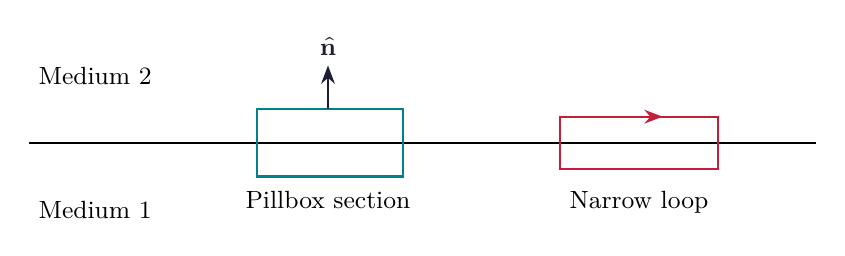
\begin{tikzpicture}[font=\small]
\draw[thick] (0,0)--(10,0);
\node[anchor=west] at (0,.85) {Medium 2};
\node[anchor=west] at (0,-.85) {Medium 1};
\draw[thick,myteal] (2.9,-.43) rectangle (4.75,.43);
\draw[arrow] (3.8,.43)--(3.8,.98) node[above] {$\hat{\mathbf n}$};
\node[below] at (3.8,-.49) {Pillbox section};
\draw[thick,myred] (6.75,-.33) rectangle (8.75,.33);
\draw[redarrow] (7.25,.33)--(8.05,.33);
\node[below] at (7.75,-.49) {Narrow loop};
\end{tikzpicture}
\end{tcolorbox}

Take $\hat{\mathbf n}$ from medium 1 to 2, free sheet charge $\rho_s$ in $\mathrm{C/m^2}$ and sheet current $\mathbf K_s$ in $\mathrm{A/m}$.
\begin{enumerate}[leftmargin=*,itemsep=3pt]
\item \textbf{Normal jumps.} Shrink the pillbox height so only cap flux remains. Opposite cap normals produce $\hat{\mathbf n}\cdot(\mathbf D_2-\mathbf D_1)=\rho_s$ and $\hat{\mathbf n}\cdot(\mathbf B_2-\mathbf B_1)=0$.
\item \textbf{Tangential jumps.} Take a loop of length $L$ along $\hat{\mathbf t}$ in medium 2 and back in medium 1. In Amp\`ere--Maxwell, as its height shrinks, $L(\mathbf H_2-\mathbf H_1)\cdot\hat{\mathbf t}=L\mathbf K_s\cdot(\hat{\mathbf n}\times\hat{\mathbf t})$. This gives $\hat{\mathbf n}\times(\mathbf H_2-\mathbf H_1)=\mathbf K_s$. In Faraday's law the flux term vanishes with the loop area, so $\hat{\mathbf n}\times(\mathbf E_2-\mathbf E_1)=0$.
\item \textbf{Perfect electric conductor (PEC).} Take zero time-harmonic fields inside and a normal pointing out of the conductor. Outside, $\mathbf E_t=0$, $B_n=0$, $D_n=\rho_s$ and $\hat{\mathbf n}\times\mathbf H=\mathbf K_s$.
\end{enumerate}

\begin{tcolorbox}[examplebox,title={Normal and tangential electric fields}]
At $z=0$, $\epsilon_1=2\epsilon_0$, $\epsilon_2=5\epsilon_0$ and $\rho_s=0$. For $\mathbf E_1=3\hat{\mathbf x}+4\hat{\mathbf z}\,\mathrm{V/m}$, $E_{2x}=E_{1x}=3\,\mathrm{V/m}$ but $E_{2z}=(\epsilon_1/\epsilon_2)E_{1z}=1.6\,\mathrm{V/m}$. It is the normal $\mathbf D$ that remains continuous.
\end{tcolorbox}

\newpage
\begin{center}
  {\large\bfseries\color{myred} Quick Revision --- Module 1}\\[3pt]
  {\small\color{mydark} Vectors, Maxwell Equations and Boundaries $|$ EC501}
\end{center}
\noindent{\color{myred}\rule{\linewidth}{1.2pt}}
\begin{tcolorbox}[formulabox,title={Key Formulas at a Glance}]
\renewcommand{\arraystretch}{1.35}
\begin{tabularx}{\linewidth}{B{5.0cm}Y}
Gauss laws & $\nabla\cdot\mathbf D=\rho_v$, $\nabla\cdot\mathbf B=0$ \\[3pt]
Faraday & $\nabla\times\mathbf E=-\partial_t\mathbf B$ \\[3pt]
Amp\`ere--Maxwell & $\nabla\times\mathbf H=\mathbf J+\partial_t\mathbf D$ \\[3pt]
Continuity & $\nabla\cdot\mathbf J=-\partial_t\rho_v$ \\[3pt]
Average flux & $\tfrac12\operatorname{Re}(\mathbf E\times\mathbf H^*)$ for peak phasors \\[3pt]
\end{tabularx}
\end{tcolorbox}
\begin{tcolorbox}[defbox,title={One-Line Definitions}]
\textbf{Gradient.} Vector pointing in the direction of steepest increase of a scalar.\par
\textbf{Displacement current density.} Time derivative of electric flux density.\par
\textbf{Poynting vector.} Directed electromagnetic power transmitted per unit area.\par
\end{tcolorbox}
\begin{tcolorbox}[exambox,title={Frequently Asked / Viva Questions}]
\begin{enumerate}[topsep=0pt, label=\textbf{Q\arabic*.}, itemsep=5pt]
\item \Q{What is the divergence theorem used for?}
Convert closed-surface outward flux to a volume integral.
\item \Q{What is the use of Stokes' theorem?}
Convert loop circulation to a surface integral of curl.
\item \Q{What is zero in magnetic Gauss law?}
Net magnetic flux through a closed surface.
\item \Q{What does Faraday's minus sign mean?}
Induction has a direction that opposes the flux change.
\item \Q{What crosses an ideal capacitor gap?}
Displacement current $dQ/dt$, associated with the changing field.
\item \Q{How is charge continuity obtained?}
Take divergence of Amp\`ere--Maxwell and use electric Gauss law.
\item \Q{Why is the magnetic phasor conjugated in average power?}
Averaging the real fields retains their relative phase.
\item \Q{What jumps across a sheet with free charge?}
The normal component of $\mathbf D$, by $\rho_s$.
\item \Q{What causes a tangential magnetic field jump?}
A free surface current $\mathbf K_s$.
\item \Q{Which electric component is zero at a PEC wall?}
The tangential component at its surface.
\end{enumerate}
\end{tcolorbox}
\begin{tcolorbox}[tikzbox,title={Summary comparison}]
\begin{tabularx}{\linewidth}{|B{4cm}|Y|}\hline
\textbf{Case} & \textbf{What to use} \\ \hline
Pillbox & Normal $\mathbf D$ and $\mathbf B$. \\ \hline
Narrow loop & Tangential $\mathbf E$ and $\mathbf H$. \\ \hline
Energy balance & Inward flux supplies stored energy increase and work on currents. \\ \hline
\end{tabularx}
\end{tcolorbox}
\end{document}
